\section{D. Irga B. Naufal Fakhri}
\subsection{Pemahaman Teori}
\begin{enumerate}
\item Device Manager pada Windows dan folder /dev pada Linux

Device manager adalah system tools yang fungsinya untuk mengidentifikasi dan mengelola hardware serta driver yang diperlukan oleh hardware yang dihubungkan. Device Manager juga bisa mengenali hardware dan menginstall drivernya secara otomatis, tapi kalo driver dari hardware tersebut tidak ada pada koleksi driver Windows, maka Device Manager akan memberikan notifikasi dan tanda khusus bahwa hardware tersebut membutuhkan driver terpisah agar bisa terinstall dengan benar.

/dev pada Linux merupakan direktori yang berfungsi untuk menyimpan konfigurasi device atau hardware dari sistem, seperti harddisk (hda, sda), terminal (tty) dll.

\item Jelaskan langkah-langkah instalasi driver dari arduino

Apabila anda menggunakan Arduino versi original maka drivernya akan diinstall saat anda menginstall Arduino IDE saat anda menhubungkan Arduino anda ke PC menggunakan kabel USB. Jika anda menggunakan Arduino Uno SMD Clone seperti saya maka anda harus menginstall drivernya terlebih dahulu setelah menginstall Arduino Uno, Caranya:
	\begin{itemize}
	\item Buka program setup.exe pada folder DRIVER1
	\begin{figure}[ht!]
		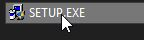
\includegraphics[width=5cm]{figures/5/1174066/0.jpg}
		\centering
		\caption{Setup}
	\end{figure}
	
	\item Setelah itu klik Install
	\begin{figure}[ht!]
		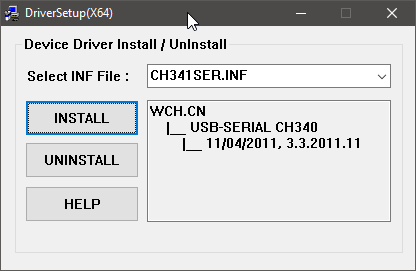
\includegraphics[width=5cm]{figures/5/1174066/1.png}
		\centering
		\caption{Instalasi}
	\end{figure}

	\item Setelah muncul seperti dibawah ini tekan OK
	\begin{figure}[ht!]
		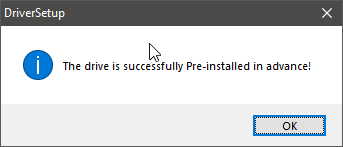
\includegraphics[width=5cm]{figures/5/1174066/2.png}
		\centering
		\caption{Instalasi Berhasil}
	\end{figure}

	\item Hubungkan Arduino ke PC, lalu buka device manager\begin{figure}[ht!]
		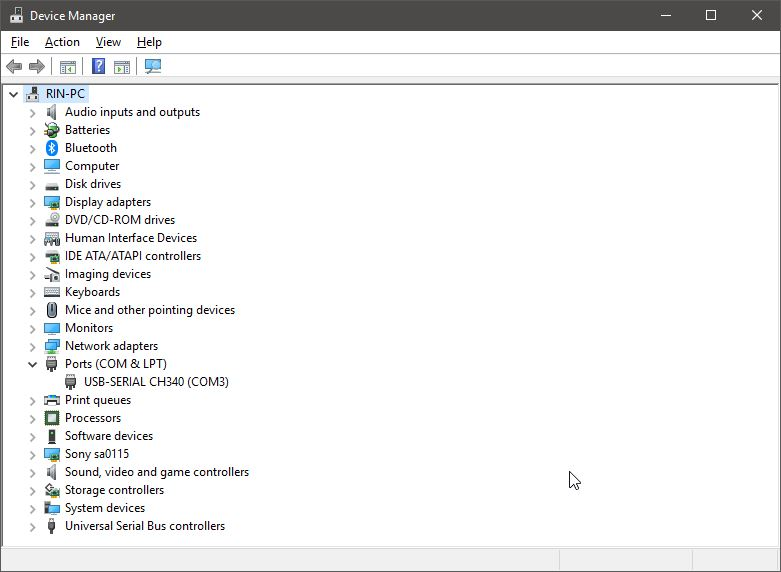
\includegraphics[width=5cm]{figures/5/1174066/3.jpg}
		\centering
		\caption{Device Manager}
	\end{figure}

	\item Lalu pilih pada bagian port apabila seperti ini maka driver arduino telah terinstall\begin{figure}[ht!]
		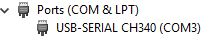
\includegraphics[width=5cm]{figures/5/1174066/4.jpg}
		\centering
		\caption{Arduino Terdeteksi}
	\end{figure}
	
	\end{itemize}

\item Jelaskan bagaimana cara membaca baudrate dan port dari komputer yang sudah terinstall driver

Cara membaca baudrate adalah dengan cara membuka arduino ide lalu mengclik serial monitor yang iconnya seperti kaca pembesar(Cari). 
Untuk mengecek port kita bisa melihatnya melalu device manager pada bagian ports, yang ada tulisan COMXX (XX adalah angka dari COM) itu adalah portnya
	
\item Jelaskan sejarah library pyserial

pySerial adalah modul API Python untuk mengakses port serial. pySerial menyediakan API yang seragam di berbagai sistem operasi, termasuk Windows, Linux, dan BSD.

\item Jelaskan fungsi-fungsi apa saja yang dipakai dari library pyserial

	\begin{itemize}
	\item Serial()
	
	Berfungsi untuk membuka port serial.
	
	\item Write()
	
	Berfungsi untuk mengirimkan data string ke port serial dan mengembalikan nomor bytes yang terkirim.
	
	\item Read(size)
	
	Berfungsi untuk membaca data dari port serial.
	
	\item Readline(size)
	
	Berfungsi untuk membaca line sampai line terakhir (EOL). 
	
	\item Close()
	
	Berfungsi untuk menutup pembacaan port serial.
	\end{itemize}

\item Jelaskan kenapa butuh perulangan dan tidak butuh perulangan dalam membaca serial

Perulangan dalam python berfungsi untuk mengulangi kode/perintah yang ada didalam perulangan tersebut. ada dua macam perulangan pada python, yang pertama for dan yang kedua while.
Perbedaan for dan while adalah for yaitu perulangan yang menghitung (Counted Loop) sedangkan while adalah perulangan yang tidak terhitung (Uncounted Loop). Penggunakan for itu biasanya jika untuk mengulangi kode yang akan ditentukan berapa kali diulangnya sedangkan while digunakan jika ada syarat tertentu untuk mengulangi kode itu dan tidak menentu berapa banyak perulangannya.
Mengapa diperlukan perulangan, karena agar data yang dibaca tidak hanya satu kali saja namun berkali kali, dengan adanya perulangan kita bisa membaca datanya berulang kali. Sehingga data yang kita baca dapat muncul lebih dari satu. Sedangkan kalau kita tidak memakai perulangan maka data yang muncul hanya satu.

\item Jelaskan bagaimana cara membuat fungsi yang mengunakan pyserial

Pembuatan fungsi sama seperti pembuatan fungsi seperti biasanya namun method dari pyserial dimasukkan kedalam fungsi dan dipanggil fungsi yang kita buat tadi
\lstinputlisting[firstline=7, lastline=14]{src/5/1174066/Teori/1174066.py}

\item Scan Plagiarisme
\begin{figure}[ht!]
	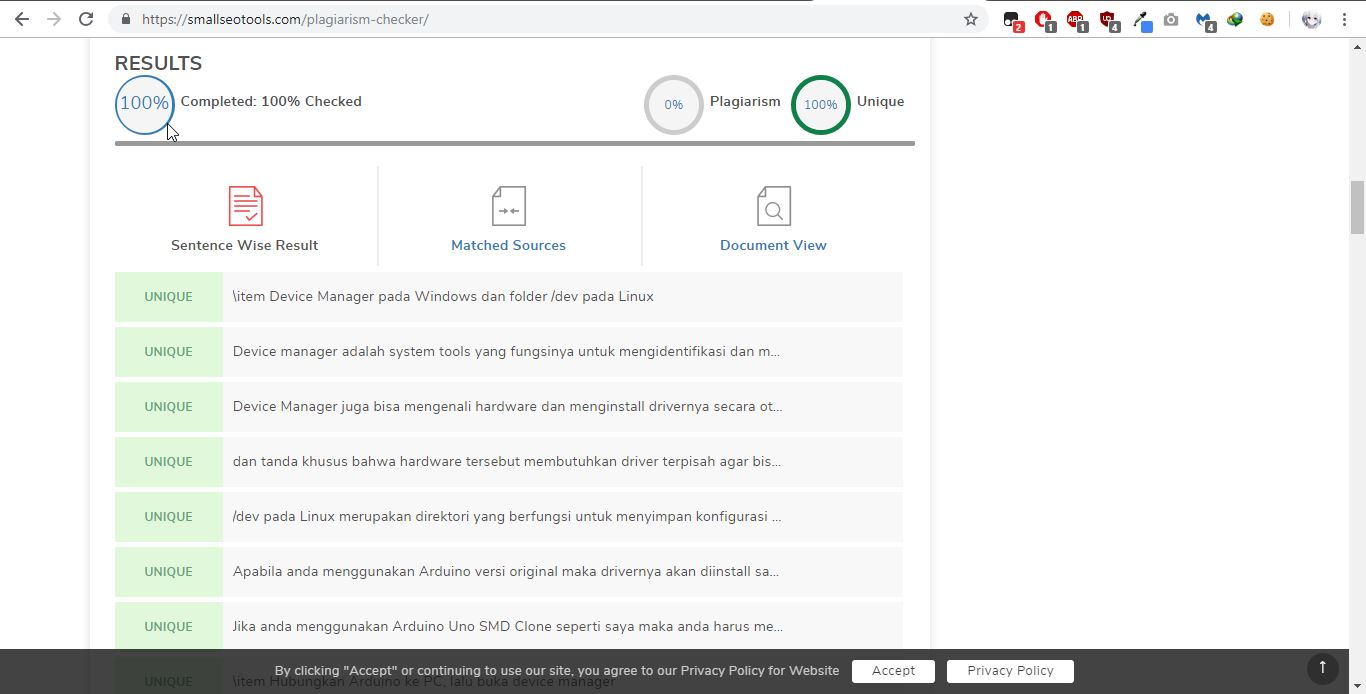
\includegraphics[width=5cm]{figures/5/1174066/plagiat.jpg}
	\centering
	\caption{Plagiarisme}
\end{figure}
\end{enumerate}

%%%%%%%%%%%%%%%%%%%%%%%%%%%%%%%%%%%%%%%%%%%%%%%%%%%%%%%%%%%%%%%%%%%%%%%%%
\section{Difa Al Fansha}
\subsection{Soal Nomor 1}
Apa itu fungsi device manager di windows dan folder /dev di linux?\\
Jawab :
\begin{itemize}
\item Fungsi Device Manager di Sistem Operasi Windows
\end{itemize}
Device manager merupakan program yang mengatur device atau perangkat yang terhuung dengan komputer / laptop.
\begin{itemize}
\item Fungsi Folder /dev di Sistem Operasi Linux
\end{itemize}
Device manager pada linux berada pada folder /dev yang mempunyai arti device. folder ini berisi konfigurasi device pada sistem.

\subsection{Soal Nomor 2}
Jelaskan langkah-langkah instalasi driver dari arduino!\\
Jawab :
\begin{enumerate}
\item Download Software IDE Arduino di https://www.arduino.cc/en/Main/Software
\item Setelah di download jalankan software tersebut.

\item Pilih I Agree.
\begin{figure}[!htbp]
  \centering
  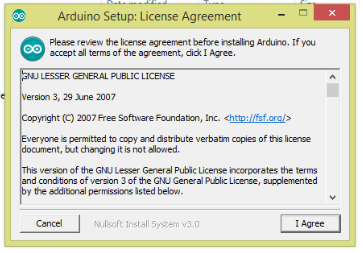
\includegraphics[height=8cm]{figures/5/1174076/Teori/1.PNG}
  \caption{Licence Agreement}
\end{figure}

\item Lalu Next.
\begin{figure}[!htbp]
  \centering
  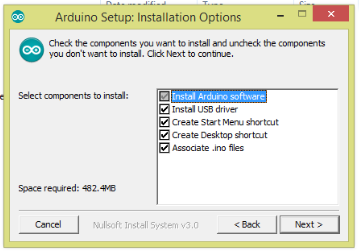
\includegraphics[height=8cm]{figures/5/1174076/Teori/2.PNG}
  \caption{Installation Options}
\end{figure}

\item Pilih directory, lalu tekan Install.
\begin{figure}[!htbp]
  \centering
  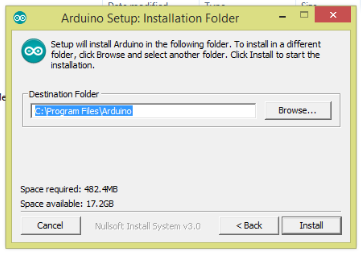
\includegraphics[height=8cm]{figures/5/1174076/Teori/3.PNG}
  \caption{Installation Folder}
\end{figure}

\item Tunggu hingga proses selesai
\begin{figure}[!htbp]
  \centering
  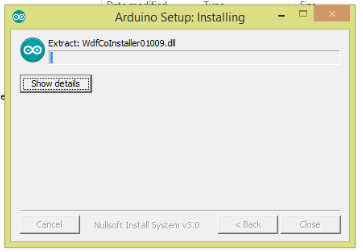
\includegraphics[height=8cm]{figures/5/1174076/Teori/4.PNG}
  \caption{Installation }
\end{figure}

\item Jika sudah selesai, tekan close
\begin{figure}[!htbp]
  \centering
  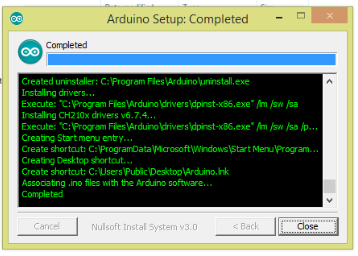
\includegraphics[height=8cm]{figures/5/1174076/Teori/5.PNG}
  \caption{Installing}
\end{figure}
\end{enumerate}

\subsection{Soal Nomor 3}
Jelaskan bagaimana cara membaca baud rate dan port dari komputer yang sudah
terinstall driver! \\
Jawab :\\
baud rate dan port akan langsung terbaca saat arduino dicolokkan ke komputer, sistem akan membaca informasi device yang terhubung.

\subsection{Soal Nomor 4}
Jelaskan sejarah library pyserial!
Jawab : \\
Salah satu cara untuk melakukan komunikasi melalui serial menggunakan python adalah dengan menggunakan modul pyserial. PySerial diluncurkan pada tahun 2002.

\subsection{Soal Nomor 5}
Jelaskan fungsi-fungsi apa saja yang dipakai dari library pyserial!\\
Jawab :\\
\begin{itemize}
\item stop() berguna untuk menghentikan program yang berjalan.
\item readline() berguna untuk membaca sebuah string dari port serial.
\item read(size)berguna untuk membaca jumlah byte dari port serial.
\item close()berguna untuk menutup port serial.
\end{itemize}

\subsection{Soal Nomor 6}
Jelaskan kenapa butuh perulangan dan tidak butuh perulangan dalam membaca serial!\\
Jawab :\\
\begin{itemize}
\item Perulangan
\end{itemize}
Perulangan diperlukan untuk untuk mengulangi perintah agar lebih mudah dan tidak terjadi penumpukan kodingan. Perulangan dijalankan jika kondisi benar dan akan berhenti jika kondisi salah.

\begin{itemize}
\item Tidak membutuhkan perulangan
\end{itemize}
Apabila perintah dijalankan sekali, kita tidak memerlukan perulangan.

\subsection{Soal Nomor 7}
Jelaskan bagaimana cara membuat fungsi yang menggunakan pyserial!\\
Jawab :\\
Definisikan nama fungsi dengan cara def namaFungsi(): lalu masukkan isi fungsi

%%%%%%%%%%%%%%%%%%%%%%%%%%%%%%%%%%%%%%%%%%%%%%%%%%%%%%%%%%%%%%%%%%%%%%%%%%%%%%%%%%%%%%%%%%%%%%%%%%%%%%%%%%%%%%%%%%%%%%%%%%

\section{Fanny Shafira Damayanti | 1174069}
\subsection{Pemahaman Teori}
\begin{enumerate}
\item Fungsi Device manager di Windows dan folder /dev di Linux

Device Manager di Windows berfungsi untuk mengelola semua Hardware yang berada di Windows.

Folder /dev berisikan file device pada Linux.

\item Langkah-langkah Instalasi driver dari arduino

\begin{itemize}
\item Download Software Arduino IDE
\item Hubungkan port USB Arduino ke port pc.
\item setelah itu pc akan mendeteksi driver baru

\begin{figure}[ht!]
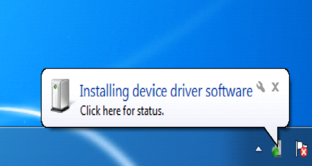
\includegraphics[width=5cm]{figures/5/1174069/1fny.png}
\centering
		\caption{Driver baru}
\end{figure}
	
\item Buka device manager

\begin{figure}[ht!]
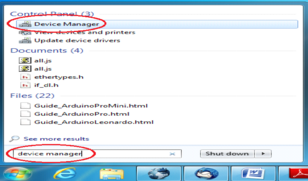
\includegraphics[width=5cm]{figures/5/1174069/2fny.png}
\centering
		\caption{Buka device manager}
\end{figure}
	
	
\item setelah itu, cari "Unknown device"

\begin{figure}[ht!]
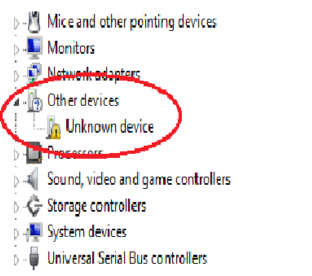
\includegraphics[width=5cm]{figures/5/1174069/3fny.png}
\centering
		\caption{klik "unknown device"}
\end{figure}
	
\item Klik kanan pada "Unknown device" lalu klik Update driver software

\begin{figure}[ht!]
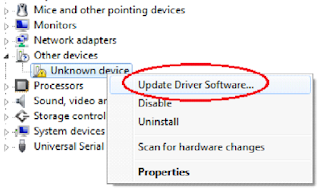
\includegraphics[width=5cm]{figures/5/1174069/4fny.png}
\centering
		\caption{Klik update driver software}
\end{figure}
	
\item Pilih Browse my computer for driver software

\begin{figure}[ht!]
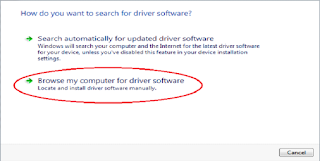
\includegraphics[width=5cm]{figures/5/1174069/5fny.png}
\centering
		\caption{Pilih browse}
\end{figure}
	
\item Cari folder installan Arduino nya

\begin{figure}[ht!]
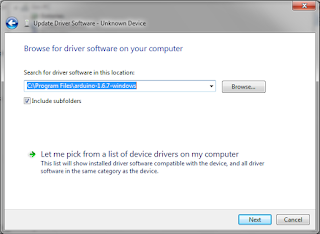
\includegraphics[width=5cm]{figures/5/1174069/6fny.png}
\centering
		\caption{Cari folder instalasinya}
\end{figure}
	
\item Lalu klik next


	
\item setelah itu klik install
\begin{figure}[ht!]
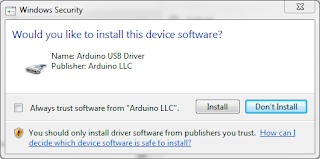
\includegraphics[width=5cm]{figures/5/1174069/7fny.png}
\centering
		\caption{install}
\end{figure}

\item Arduino telah berhasil di install

\begin{figure}[ht!]
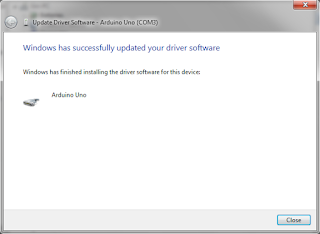
\includegraphics[width=5cm]{figures/5/1174069/8fny.png}
\centering
\caption{selesai}
\end{figure}
	
\end{itemize} 

\item Cara membaca baudrate dan port dari komputer yang sudah terinstall driver

Untuk membaca baudrate dan port yaitu dengan cara :
\begin{itemize}
\item menginstall Arduino IDE
\item setelah itu buka menu serial monitor yang berada di tab tools
\item lalu akan terlihat baudrate dan port yang sedang digunakan.
\end{itemize}

\item Sejarah library pyserial
PySerial merupakan sebuah library yang digunakan untuk komunikasi ke port serial terutama untuk mikrokontroller. PySerial pertama kali diluncurkan pada tahun 2002 yang makin berkembang dalam setiap versinya hingga tahun 2017 lalu.

\item Fungsi-fungsi yang di pakai dari libarary pyserial

\begin{itemize}
			\item \begin{verbatim}stop()\end{verbatim} : untuk menghentikan pembacaan program
			\item \begin{verbatim}serial.to_bytes(sequence)\end{verbatim} : berfungsi untuk mengubah sequence ke dalam bytes agar dapat dikirim ke dalam arduino.
			\item \begin{verbatim}close()\end{verbatim} : untuk menutup port dan menghentikan pembacaan program
		\end{itemize}

\item kenapa butuh perulangan dan tidak butuh perulangan dalam membaca serial

Karena perulangan digunakan untuk membaca seluruh data pada serial yang ada setiap baris. Perulangan digunakan agar data dapat muncul secara terus menerus atau realtime. Sedangkan kalau tidak memakai perulangan, maka data hanya muncul satu kali, tidak berulang.

\item Cara membuat fungsi menggunakan pyserial

\lstinputlisting[firstline=7, lastline=14]{src/5/1174069/Teori/1174069_teori.py}

\item Scan Plagiarisme
\begin{figure}[ht!]
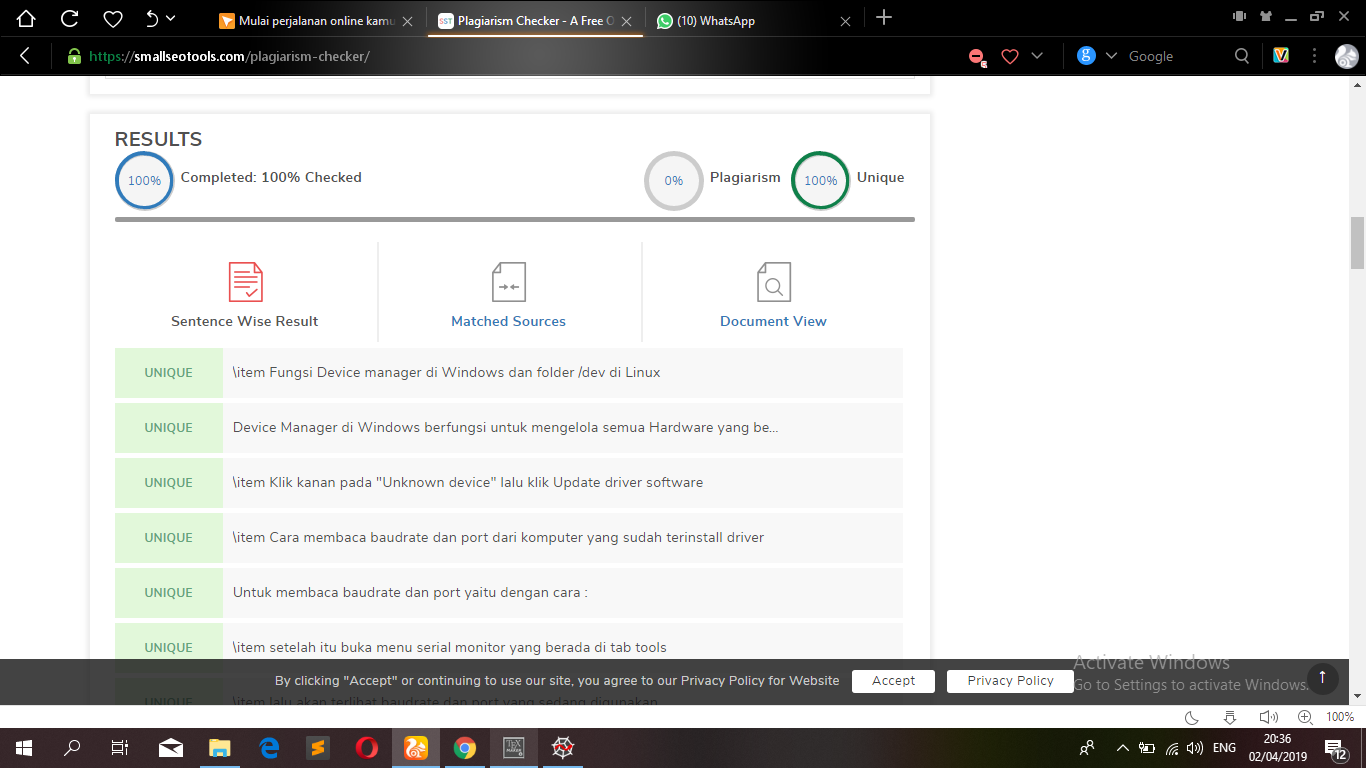
\includegraphics[width=5cm]{figures/5/1174069/plagiarisme.png}
\centering
\caption{plagiarisme}
\end{figure}
\end{enumerate}

%%%%%%%%%%%%%%%%%%%%%%%%%%%%%%%%%%%%%%%%%%%%%%%%%%%%%%%%%%%%%%%%%%%%%%%%%%%%%%%%%%%%%%%%%%%%%%%%%%%%%%%%%%%%%%%%%%%%

\section{Aulyardha Anindita | 1174054}
\subsection{Pemahaman Teori}
\begin{enumerate}

\item Fungsi Device Manager dan folder /dev
\begin{itemize}
\item Fungsi Device Manager\\
Device manager dalam windows merupakan perluasan dari microsoft management console. Device manager mampu menampilkan seluruh hardware yang bisa di inisialisasi (dikenali) oleh windows. Device manager disini memiliki beberapa fungsi diantaranya :\\
a.	Menunjukkan status suatu hardware\\
b.	Menunjukkan informasi detail suatu hardware\\
c.	Mengelola driver hardware\\
d.	Disable dan enable hardware\\
e.	Memberikan pesan error terjadinya problem status device\\
\item Fungsi Folder /dev\\
Folder/dev adalah suatu representasi dari drive yang terhubung ke dalam sistem operasi linux dan sistem mengganggapnya sebagai file-file direktori. Biasanya sering ditampilkan direktori seperti /dev/sdal yang mewakili Drive SATA pertama dalam sistem.
\end{itemize}

\item Langkah-langkah instalasi driver dari arduino
\begin{itemize}
\item Pertama, download dan instal terlebih dahulu Arduino IDE

\item Hubungkan port USB Arduino UNO ke Port USB PC, maka PC akan mendeteksi keberadaan perangkat baru dan akan muncul pop up berupa pesan install device driver software. Seperti pada gambar berikut :
\begin{figure}[ht!]
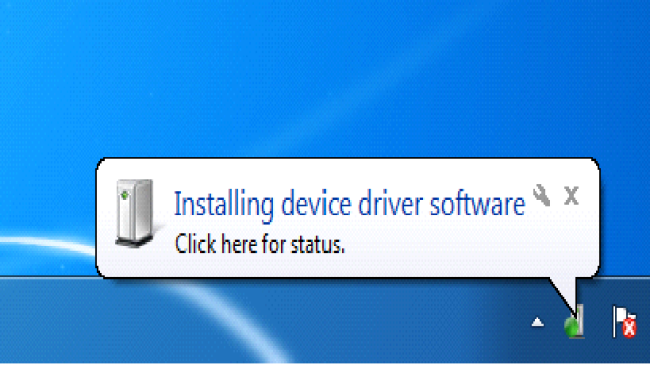
\includegraphics[width=5cm]{figures/5/1174054/1.png}
\centering
\caption{Setup}
\end{figure}

\item Dalam Windows tidak menyediakan menyediakan driver untuk Arduino Uno seperti yang terlihat pada gambar dibawah ini, sehingga proses instalasinya harus dilakukan secara manual.
\begin{figure}[ht!]
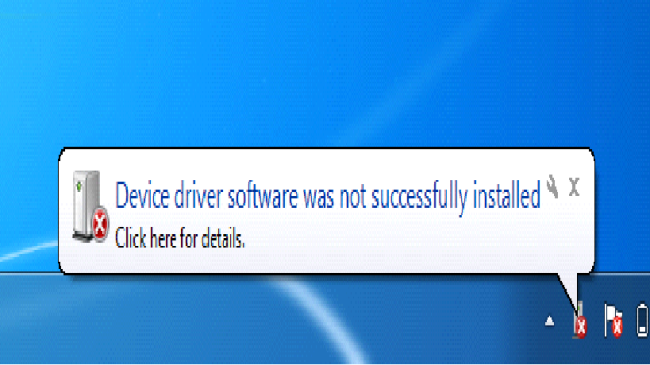
\includegraphics[width=5cm]{figures/5/1174054/2.png}
\centering
\caption{Instalasi}
\end{figure}

\item Selanjutnya, buka start windows kemudian ketikkan device manager lalu tekan enter, maka akan muncul device manager. Klik untuk menjalankan. Seperti pada gambar berikut :
\begin{figure}[ht!]
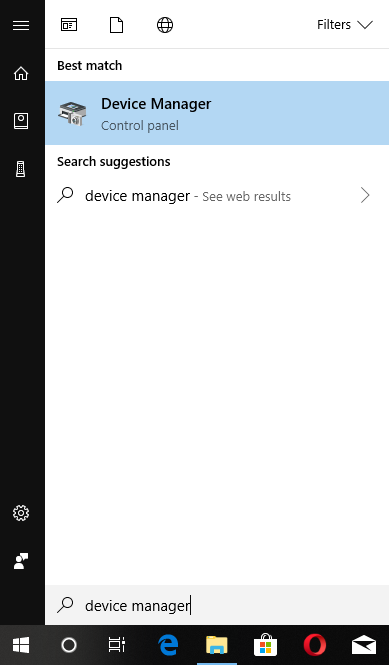
\includegraphics[width=5cm]{figures/5/1174054/3.png}
\centering
\caption{Search Device Manager}
\end{figure}

\item Kemudian Carilah Unknown device pada bagian Other device, biasanya terdapat tanda seru berwarna kuning hal itu disebabkan karena penginstallan tidak berjalan dengan sempurna.
\begin{figure}[ht!]
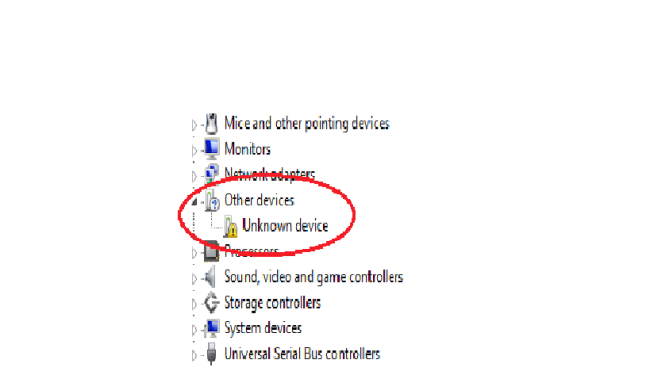
\includegraphics[width=5cm]{figures/5/1174054/4.png}
\centering
\caption{Unknown Device}
\end{figure}

\item Klik kanan pada “Unknown device” kemudian pilih Update Driver Software
\begin{figure}[ht!]
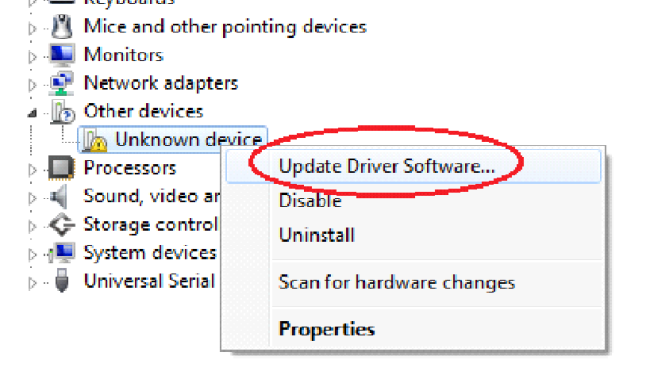
\includegraphics[width=5cm]{figures/5/1174054/5.png}
\centering
\caption{Update Driver Software}
\end{figure}

\item Pilih Browse my computer for driver software
\begin{figure}[ht!]
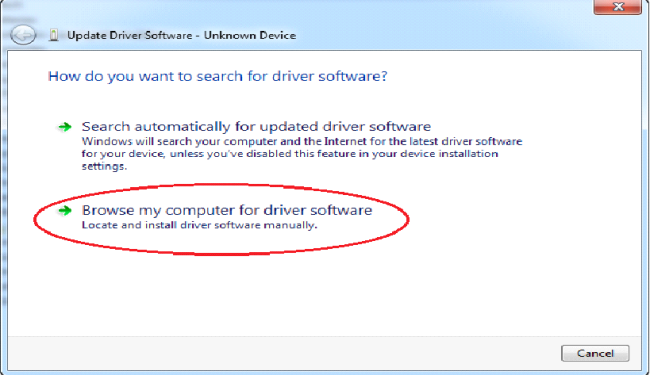
\includegraphics[width=5cm]{figures/5/1174054/6.png}
\centering
\caption{Mencari folder untuk driver software}
\end{figure}

\item  Arahkan lokasi folder ke folder arduino kemudian checkbox lalu centang include subfolders. setelah itu, Klik Next untuk melanjutkan instalasi driver.
\begin{figure}[ht!]
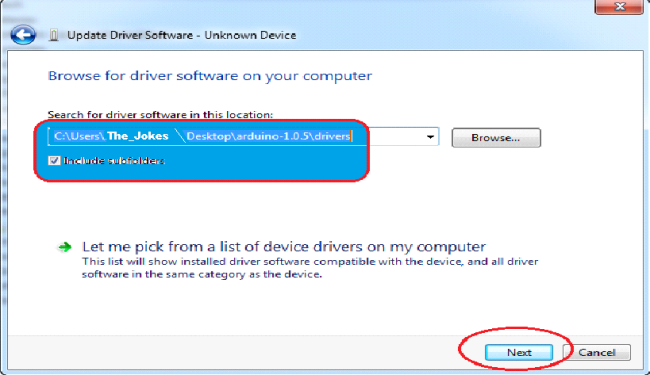
\includegraphics[width=5cm]{figures/5/1174054/7.png}
\centering
\caption{Lokasi folder}
\end{figure}

\item Kemudian lanjutkan dengan mengklik Install pada tampilan Windows Security
\begin{figure}[ht!]
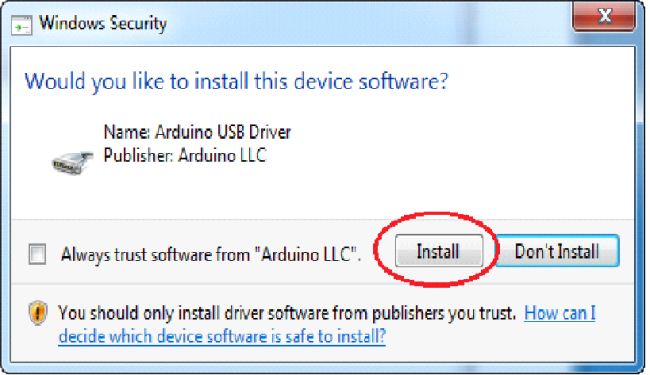
\includegraphics[width=5cm]{figures/5/1174054/8.png}
\centering
\caption{Install PAda tampilan WIndows Security}
\end{figure}

\item Jika instalasi driver berhasil maka akan muncul Windows has successfully updated your driver software.
\begin{figure}[ht!]
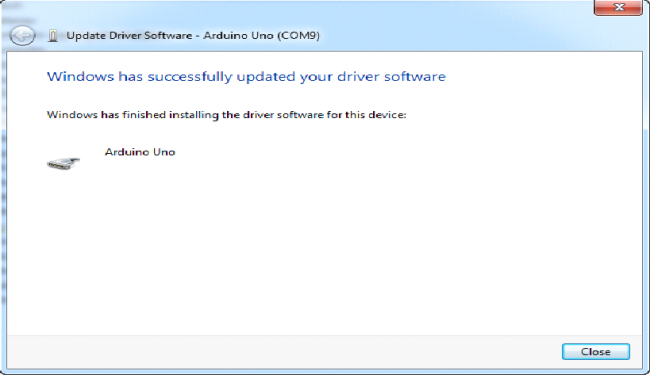
\includegraphics[width=5cm]{figures/5/1174054/9.png}
\centering
\caption{Pesan Peringatan Berhasil}
\end{figure}

\item Perhatikan dan ingat nama COM Arduino Uno, karena nama COM ini yang akan digunakan untuk meng-upload program nantinya
\begin{figure}[ht!]
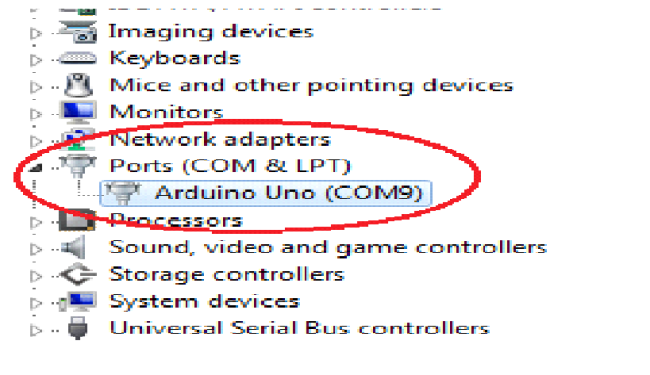
\includegraphics[width=5cm]{figures/5/1174054/10.png}
\centering
\caption{Peringatan COM Arduino Uno}
\end{figure}

\end{itemize}

\item Cara Membaca Baudrate dan Port

Cara membaca baudrate yaitu dengan membuka arduino ide yang telah diinstal lalu klik serial monitor dimana iconnya seperti kaca pembesar (cari).

Cara membaca port yaitu dengan melalui device manager pada bagian port yang terdapat tulisan COMXX dimana itu adalah portnya.

\item Sejarah Library Pyserial\\
PySerial merupakan sebuah library yang digunakan untuk komunikasi ke port serial terutama untuk mikrokontroller. PySerial pertama kali diluncurkan pada tahun 2002 yang makin berkembang dalam setiap versinya hingga tahun 2017 lalu. 

PySerial menyediakan antarmuka untuk berkomunikasi
melalui protokol komunikasi serial. Komunikasi serial adalah salah satu protokol komunikasi komputer tertua. Protokol komunikasi serial mendahului spesifikasi USB
yang digunakan oleh komputer dan perangkat keras lain seperti mouse, keyboard,dan webcam. USB adalah singkatan dari Universal Serial Bus. USB dan dibangun di atas dan memperluas antarmuka komunikasi serial asli.

\item Fungsi-fungsi pada Library Pyserial
\begin{itemize}
\item Serial(), berfungsi untuk membuka port serial
\item Write(), berfungsi untuk menulis data lewat port serial
\item readline(size), berfungsi untuk membaca sebuah string dari port serial
\item read(size), berfungsi untuk membaca jumlah byte dari port serial
\item close(), berfungsi untuk menutup port serial
\end{itemize}

\item Mengapa butuh perulangan dan tidak butuh perulangan dalam membaca serial\\
Ketika kita akan membaca serial di Arduino diperlukan perulangan yang berfungsi untuk membaca data secara berulang kali sehingga data yang muncul banyak. Sedangkan apabila tidak membutuhkan perulangan maka Arduino hanya akan membaca data satu kali saja.

\item Cara Membuat fungsi menggunakan Pyserial
\lstinputlisting[firstline=8, lastline=15]{src/5/1174054/Teori/1174054.py}

\item Cek Plagiarisme
\begin{figure}[ht!]
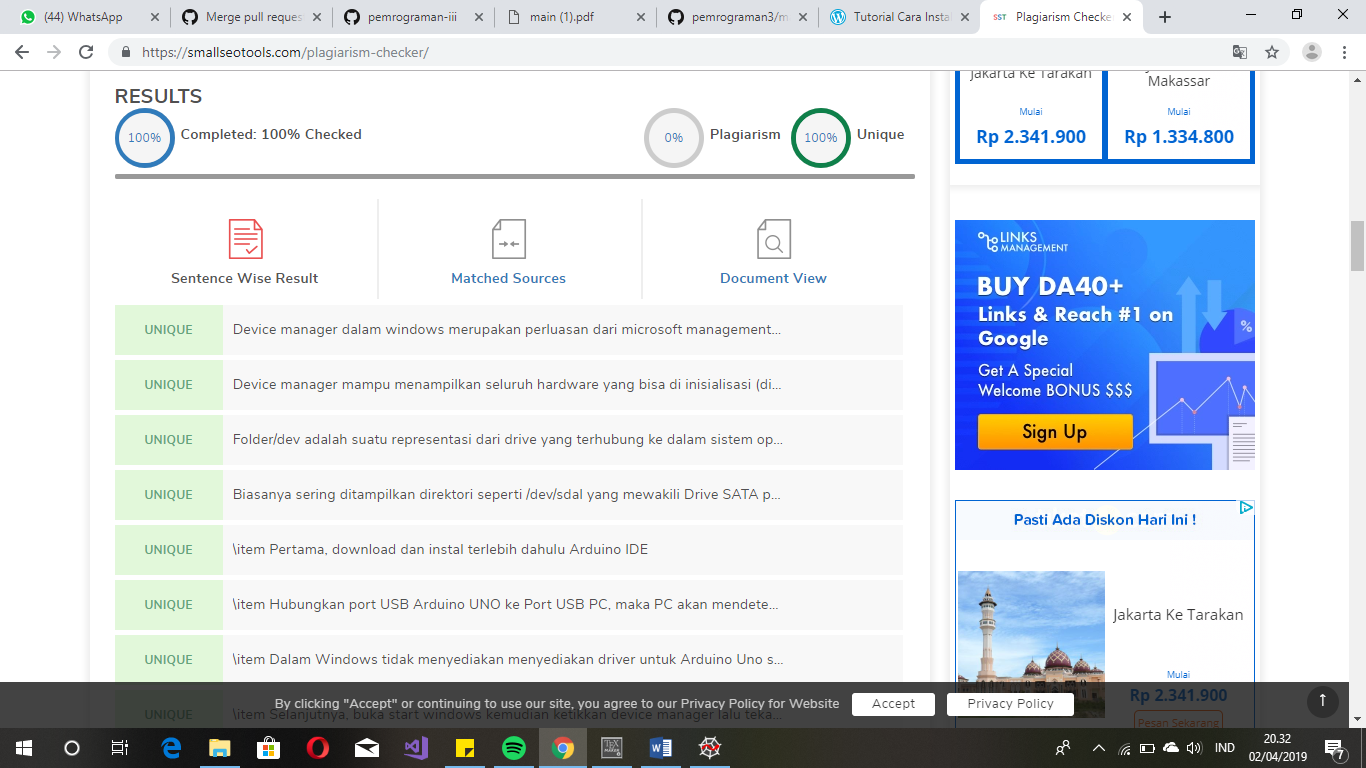
\includegraphics[width=5cm]{figures/5/1174054/plagiarisme.png}
\centering
\caption{Plagiarisme}
\end{figure}

\end{enumerate}

%%%%%%%%%%%%%%%%%%%%%%%%%%%%%%%%%%%%%%%%%%%%%%%%%%%%%%%%%%%%%%%%%%%%%%%%%%%%%%%%%%%%%%%%%%%%%%%%%%%%%%%%%%%%%%%%%%%%

\section{Nurul Izza Hamka | 1174062 | Teori}
\begin{enumerate}

\item Fungsi Device Manager di Windows dan Folder / Dev di Linux 
Device manager ini adalah untuk menampilkan semua hardware yang bisa dikenali oleh windows, tampilan di device manager ini sudah dikelompokkan dengan rapi serta teratur,dengan adanya device manager ini akan sangat membantu dalam memanajemen setiap hardware yang ada dalam windows. \\
Fungsi dari device manager ini adalah seperti :\\
1. Mengelola setiap driver didalam hardware,\\
2. Mengidentifikasi konfik yang terjadi dalam hardware,\\
3. Menunjukka setiap informasi secara detail suatu hardware,\\
4. Menampilkan status dalam hardware.\\
Sedangka pada Linux ia melihat hardware apa saja yang yang telah terpasang melalui command dan terminal ataupun secara Visual.

\item Langkah-Langkah Instalasi Driver dari Arduino : \\
Adapun langkah-langkah dalam menginstal arduino di Windows :\\
\begin{enumerate}
\item Pertama Hubungkan Port USB arduino UNO ke komputer atau Laptop,
	\item Setelah terhubung, laptop akan mengindentifikasi terlebih dahulu,
	\begin{figure}[ht!]
	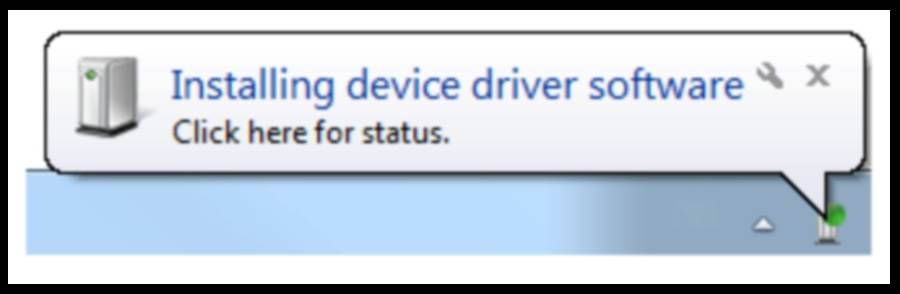
\includegraphics[width=5cm]{figures/5/1174062/1.jpg}
	\centering
	\end{figure}
	\item Selanjutnya windows akan menginstall di driver,pastikan device manager kita telah terinstall,
	\begin{figure}[ht!]
	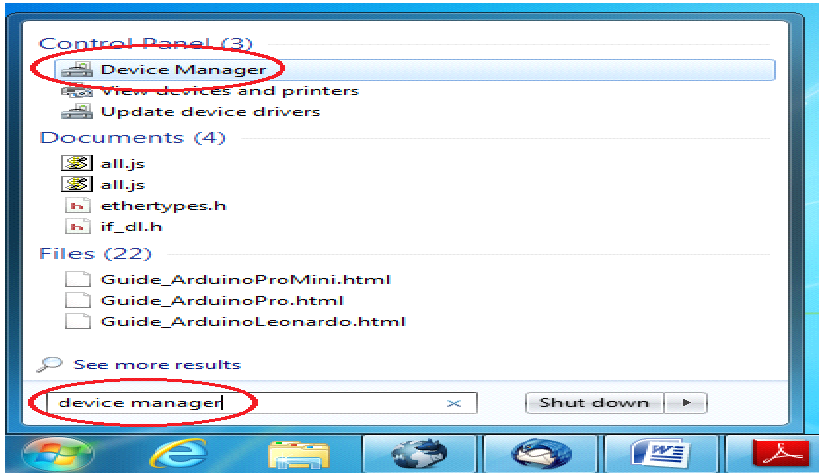
\includegraphics[width=5cm]{figures/5/1174062/2.png}
	\centering
	\end{figure}
	\item Di device manager padsa bagian Ports, akan muncul nama baru yaitu Arduino UNO,
	\item Klik kanan Arduino Uno tersebut kemudian pilih Update Driver Software, 
	\begin{figure}[ht!]
	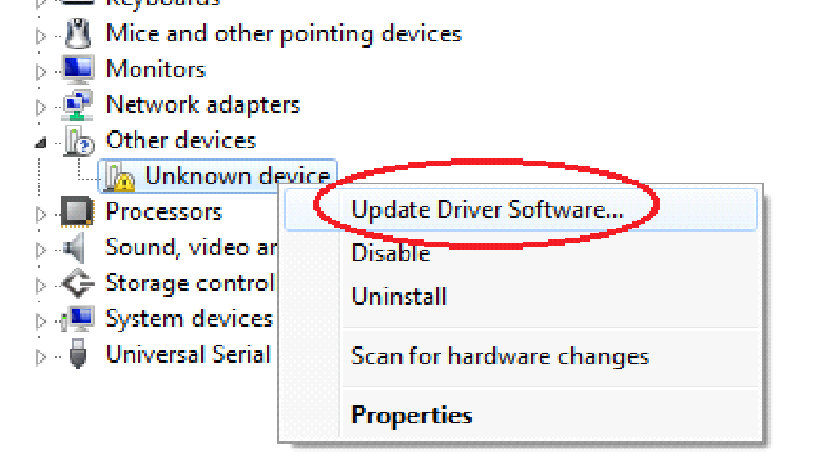
\includegraphics[width=5cm]{figures/5/1174062/4.png}
	\centering
	\end{figure}
	\item Setelah itu Browser my Computer for driver software,lalu klik Next untuk install
	\begin{figure}[ht!]
	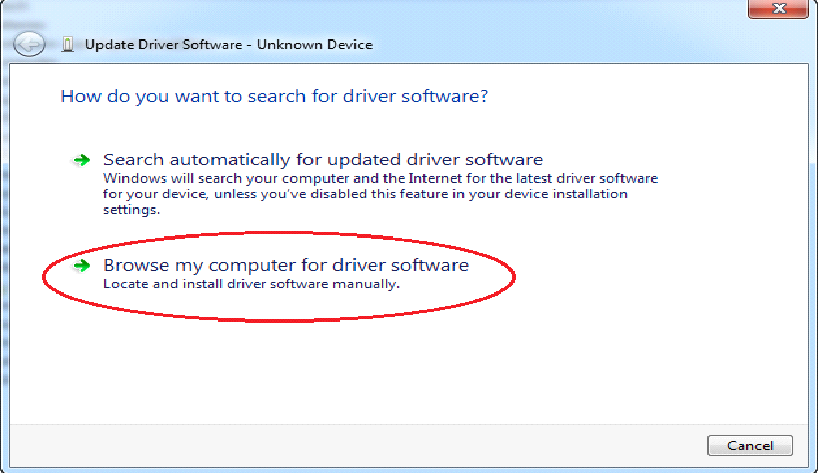
\includegraphics[width=5cm]{figures/5/1174062/5.png}
	\centering
	\end{figure}
	\item Jika berhasil, berarti Arduino telah berhasil di install.
	\begin{figure}[ht!]
	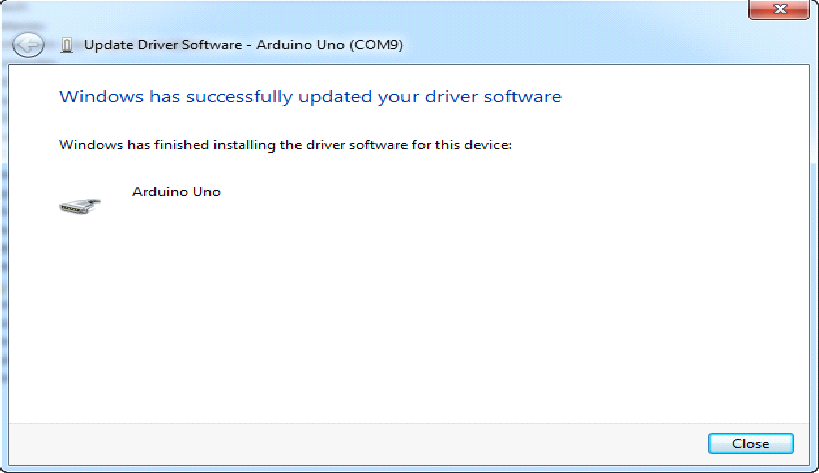
\includegraphics[width=5cm]{figures/5/1174062/7.png}
	\centering
	\end{figure}
\end{enumerate}
	

\item Cara membaca baudrate dan Port dari Komputer yang telah Terinstall Driver: \\
1. Buka device manager,\\
2. Pilih port (COM \& LPT),\\
3. Kemuadian double klik yang COM,\\
4. Pilih tab yang Port Setting, dan lihat pada Bit per Second,\\

Kemudian Cara Membaca Port Dari Komputer :
1. Buka device manager,\\
2. Pilih port (COM \& LPT),\\
3. Selanjutnya akan muncul jika port arduino telah terbaca oleh PC.\\

\item Sejarah Library Pyserial:
Pyserial adalah perpustakaan yang meyediakan  dukungan untuk sebuah koneksi serial "RS-232" melalui berbagi perangkat yang berbeda. Pyserial ini adalah paket python yang mempasilitasi komunikasi serial antara Pc dengan perngkat keras eksternal. Pyserial ini menyediakan interface yang dapat digunakan untuk berkomunikasi melalui protokol komunikasi serial. 

\item Fungsi-Fungsi Yang Dipakai Dari Library Pyserial:
1. Serial,digunakan untuk membuka port serial,\\
2. Write(data), digunakan untuk menulis data lewat port serial,\\
3. Readline(),digunakan untuk membaca sebuah string dari port serial,\\
4. Read(size),digunakan untuk membaca jumlah byte dari port serial,\\
5. Close(),digunakan untuk menutup port serial.\\

\item Kenapa Butuh Perulangan dan Tidak Butuh Perulangan Dalam Membaca Serial:

ketika membaca serial pada arduino maka akan dibutuhkan perulangan untuk bisa membaca setiap data secara berulang, sehingga data-data yang muncul bisa banyak. \\
Sedangkan jika kita tidak membutuhkan perulangan maka Arduino hanya akan membaca data sekali saja. 

\item Bagaimana Cara Membuat Fungsi Yang Menggunakan pyserial.

\item Plagiarisme
	\begin{figure}[ht!]
	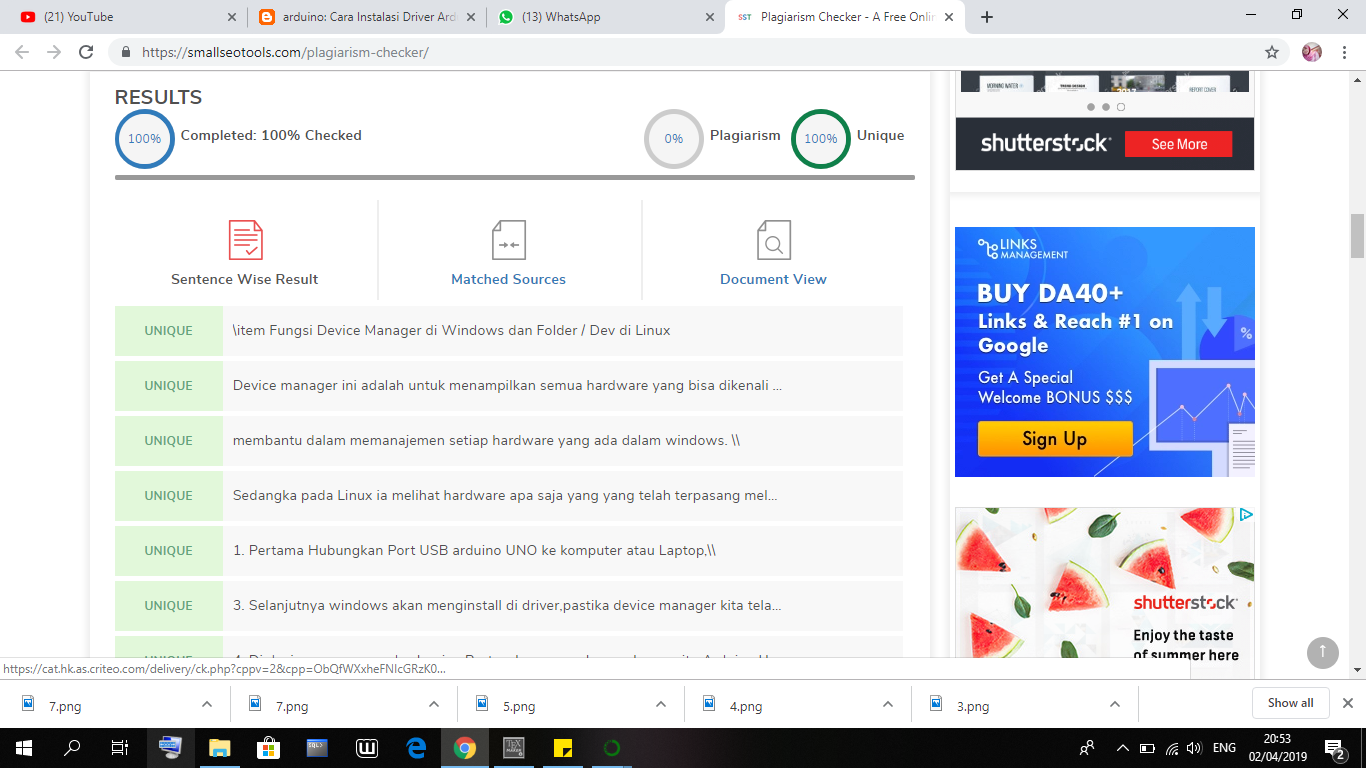
\includegraphics[width=5cm]{figures/5/1174062/8.png}
	\centering
	\end{figure}

\end{enumerate}

%%%%%%%%%%%%%%%%%%%%%%%%%%%%%%%%%%%%%%%%%%%%%%%%%%%%%%%%%%%%%%%%%%

\section{Tia Nur Candida | 1174086}
{\Large \textbf{Pemahaman Teori}}
\subsection{Soal No. 1}
Apa itu fungsi device manager di windows dan folder /dev di linux?

\hfill \break
Device manager merupakan perangkat lunak untuk menampilkan seluruh perangkat keras yang di-inisialisasi atau dikenali oleh sistem operasi Windows. Device Manager membantu dalam mengelola atau me-manage semua perangkat keras yang terpasang dan terdeteksi dalam sistem Windows. Perangkat keras tersebut bisa berupa harddisk, kartu VGA, sound, keyboard, perangkat USB dan lain-lainnya.

\hfill \break
Fungsi device manager antara lain :
\begin{enumerate}
	\item Menunjukkan status mengenai suatu perangkat keras.
	\item Menunjukkan informasi detail mengenai suatu perangkat keras.
	\item Mengelola driver perangkat keras.
	\item Menonaktifkan dan mengaktifkan perangkat keras.
	\item Mengidentifikasi konflik antar perangkat keras.
	\item Memberitahukan terjadinya masalah pada perangkat keras.
\end{enumerate}

\hfill \break
Folder /dev merupakan representasi dari drive yang terhubung ke sistem operasi Linux dan oleh sistem dianggap sebagai file-file direktori. Biasanya sering ditampilkan direktori seperti /dev/sda1 yang mewakili Drive SATA pertama dalam sistem.

\subsection{Soal No. 2}
Jelaskan langkah-langkah instalasi driver dari arduino!

\hfill \break
Berikut ini adalah langkah-langkah instalasi driver dari Arduino UNO di Windows:

\begin{enumerate}
	\item Pertama pastikan Arduino IDE telah terinstall.
	\item Lalu hubungkan port USB Arduino Uno ke port USB PC.
	\item Kemudian PC anda akan mendeteksi perangkat baru yang terpasang dan akan muncul pop seperti ini.
	\begin{figure}[H]
		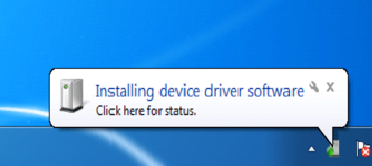
\includegraphics[width=10cm]{figures/5/1174086/Teori/1.png}
		\centering
	\end{figure}
	\item Karena Arduino Uno baru pertama kali terpasang, maka akan muncul pop up error seperti ini.
	\begin{figure}[H]
		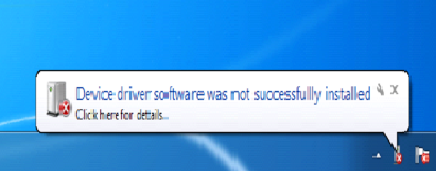
\includegraphics[width=10cm]{figures/5/1174086/Teori/2.png}
		\centering
	\end{figure}
	\item Buka ''Start'' lalu cari Device Manager, kemudian klik ''Device Manager''.
	\begin{figure}[H]
		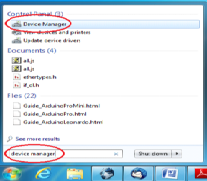
\includegraphics[width=10cm]{figures/5/1174086/Teori/3.png}
		\centering
	\end{figure}
	\item Setelah Device Manager terbuka, silahkan cari ''Unknown Device'' yang berada di Other Device.
	\begin{figure}[H]
		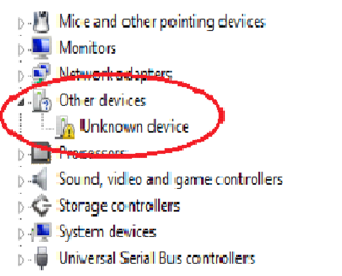
\includegraphics[width=10cm]{figures/5/1174086/Teori/4.png}
		\centering
	\end{figure}
	\item Kemudian klik kanan pada ''Unknown Device'', lalu pilih ''Update Driver Software''.
	\begin{figure}[H]
		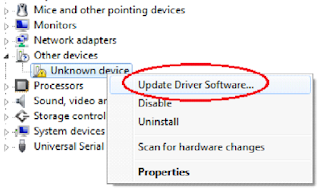
\includegraphics[width=10cm]{figures/5/1174086/Teori/5.png}
		\centering
	\end{figure}
	\item Setelah itu muncul window baru, lalu pilih ''Browse my computer for driver software''.
	\begin{figure}[H]
		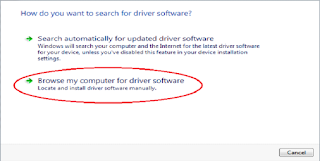
\includegraphics[width=10cm]{figures/5/1174086/Teori/6.png}
		\centering
	\end{figure}
	\item Lalu cari folder yang terinstall Arduino IDE dengan mengklik browse. Kemudian klik ''Next''.
	\begin{figure}[H]
		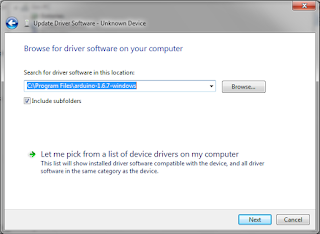
\includegraphics[width=10cm]{figures/5/1174086/Teori/7.png}
		\centering
	\end{figure}
	\item Windows akan mencari dan menginstall driver yang berada pada folder tersebut.
	\begin{figure}[H]
		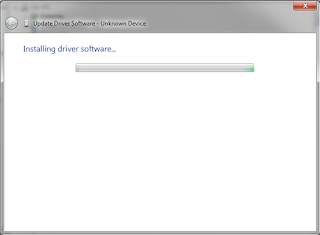
\includegraphics[width=10cm]{figures/5/1174086/Teori/8.png}
		\centering
	\end{figure}
	\item Setelah itu akan muncul window, lalu klik ''Install''.
	\begin{figure}[H]
		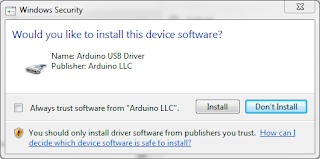
\includegraphics[width=10cm]{figures/5/1174086/Teori/9.png}
		\centering
	\end{figure}
	\item Jika berhasil terinstal maka akan muncul window seperti ini.
	\begin{figure}[H]
		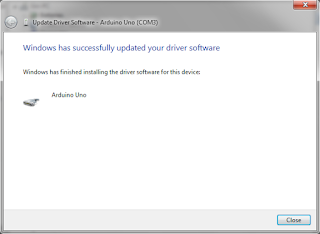
\includegraphics[width=10cm]{figures/5/1174086/Teori/10.png}
		\centering
	\end{figure}
\end{enumerate}

\subsection{Soal No. 3}
Jelaskan bagaimana cara membaca baudrate dan port dari komputer yang sudah terinstall driver!

\hfill \break
\textbf{Membaca Baudrate dari Komputer}
\begin{enumerate}
	\item Pertama buka ''Start''. Cari ''Device Manager'', lalu klik.
	\begin{figure}[H]
		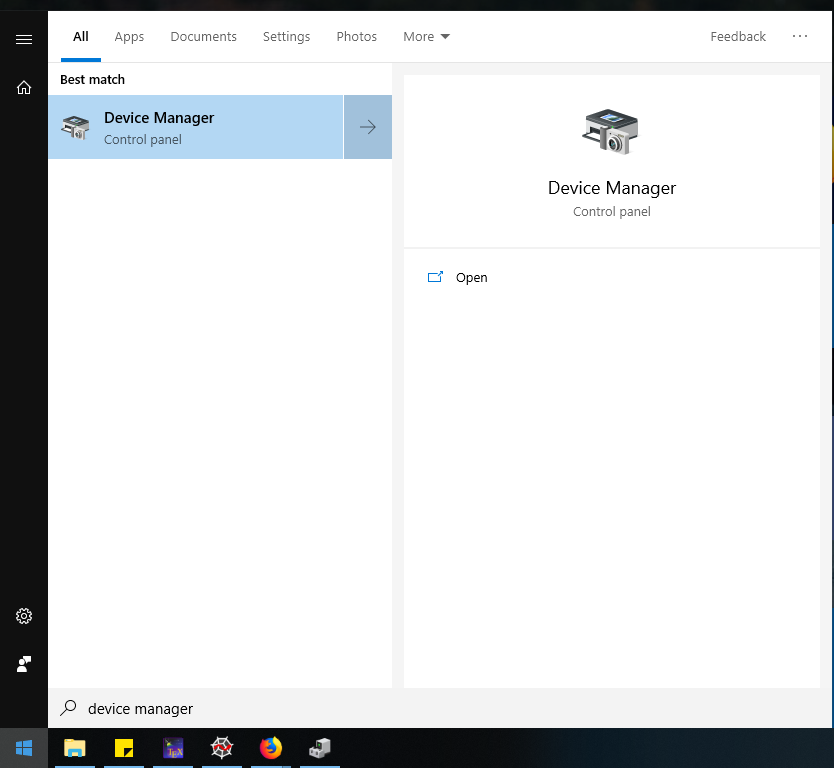
\includegraphics[width=10cm]{figures/5/1174086/Teori/d1.png}
		\centering
	\end{figure}
	
	\item Kemudian pilih ''Ports (COM \& LPT)''.
	\begin{figure}[H]
		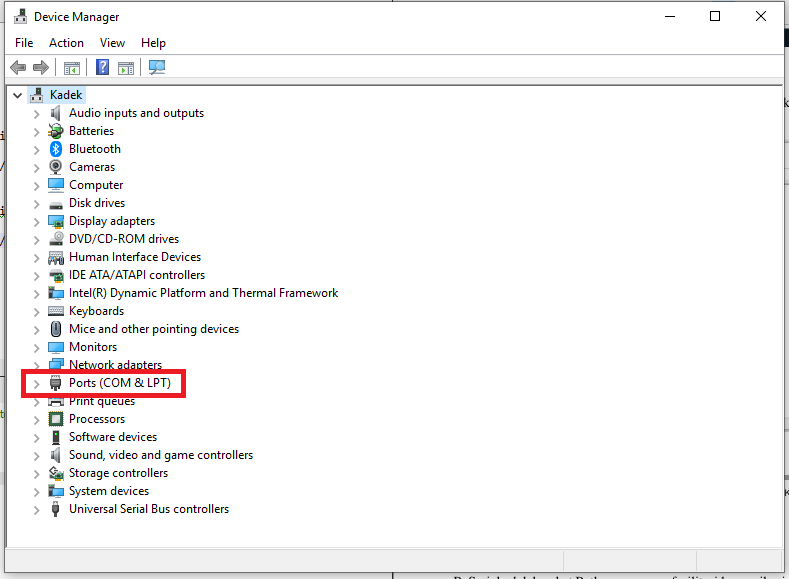
\includegraphics[width=10cm]{figures/5/1174086/Teori/d3.png}
		\centering
	\end{figure}
	
	\item Klik dua kali pada COM yang terhubung.
	\begin{figure}[H]
		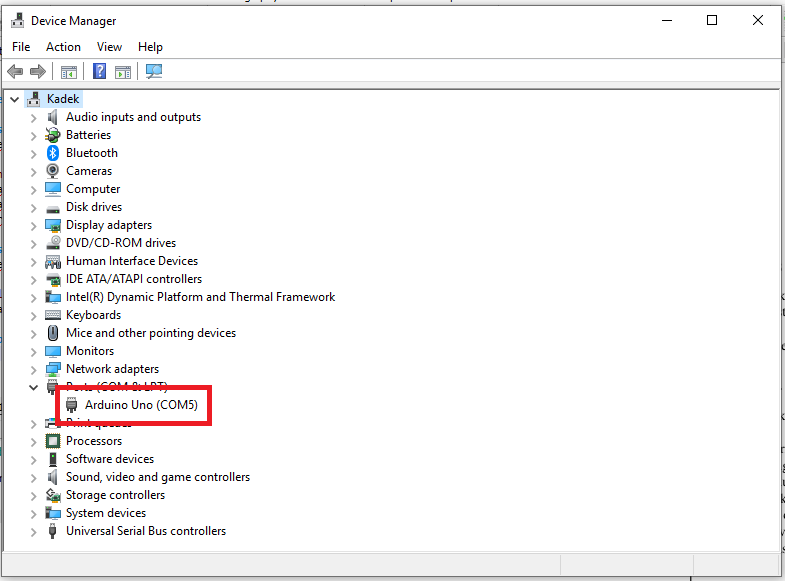
\includegraphics[width=10cm]{figures/5/1174086/Teori/d2.png}
		\centering
	\end{figure}

	\item Pilih tab ''Port Settings'', lalu lihat di ''Bit per second''.
	\begin{figure}[H]
		\includegraphics[width=8cm]{figures/5/1174086/Teori/d4.png}
		\centering
	\end{figure}
\end{enumerate}


\hfill \break
\textbf{Membaca Port dari Komputer}

\begin{enumerate}
	\item Pertama buka ''Start''. Cari ''Device Manager'', lalu klik.
	\begin{figure}[H]
		\includegraphics[width=10cm]{figures/5/1174086/Teori/d1.png}
		\centering
	\end{figure}

	\item Kemudian pilih ''Ports (COM \& LPT)''.
	\begin{figure}[H]
		\includegraphics[width=10cm]{figures/5/1174086/Teori/d3.png}
		\centering
	\end{figure}

	\item Port dari Arduino telah terbaca oleh PC.
	\begin{figure}[H]
		\includegraphics[width=10cm]{figures/5/1174086/Teori/d2.png}
		\centering
	\end{figure}
\end{enumerate}



\subsection{Soal No. 4}
Jelaskan sejarah library pyserial!

\hfill \break
PySerial adalah paket Python yang menfasilitasi komunikasi serial antara PC dengan perangkat keras eksternal. PySerial menyediakan antarmuka untuk berkomunikasi melalui protokol komunikasi serial. Komunikasi serial adalah salah satu protokol komunikasi komputer tertua. Protokol komunikasi serial mendahului spesifikasi USB yang digunakan oleh komputer dan perangkat keras lain seperti mouse, keyboard, dan webcam. USB adalah singkatan dari Universal Serial Bus. USB dan dibangun di atas dan memperluas antarmuka komunikasi serial asli.

\subsection{Soal No. 5}
Jelaskan fungsi-fungsi apa saja yang dipakai dari library pyserial!

\hfill \break
Fungsi-fungsi yang dipakai dari library PySerial, yaitu:
\begin{enumerate}
	\item Serial - fungsi ini untuk membuka port serial.
	\item write(data) - fungsi ini menulis data lewat port serial.
	\item readline() - fungsi ini membaca sebuah string dari port serial.
	\item read(size) - fungsi ini untuk membaca jumlah byte dari port serial.
	\item close() - fungsi ini untuk menutup port serial.
\end{enumerate}

\subsection{Soal No. 6}
Jelaskan kenapa butuh perulangan dan tidak butuh perulangan dalam membaca serial!

\hfill \break
Pada saat membaca serial di Arduino diperlukan perulangan agar bisa membaca data secara berulang kali sehingga data yang muncul banyak. Sedangkan apabila tidak membutuhkan perulangan maka Arduino hanya akan membaca data sekali saja.

\subsection{Soal No. 7}
Jelaskan bagaimana cara membuat fungsi yang mengunakan pyserial!

\lstinputlisting[caption = Fungsi yang menggunakan pyserial., firstline=1, lastline=7]{src/5/1174086/1174086.py}

\begin{figure}[H]
	\includegraphics[width=10cm]{figures/5/1174086/Teori/hasil.png}
	\centering
	\caption{Hasil pembuatan fungsi pyserial.}
\end{figure}

\subsection{Cek Plagiat}
\begin{figure}[H]
	\includegraphics[width=10cm]{figures/5/1174086/Teori/plagiat.png}
	\centering
	\caption{Hasil cek plagiat.}
\end{figure}

\subsection{Kode Program}
\begin{figure}[H]
	\includegraphics[width=10cm]{figures/5/1174086/Teori/kodeprogram.png}
	\centering
	\caption{Kode program file 1174086.py.}
\end{figure}
%%%%%%%%%%%%%%%%%%%%%%%%%%%%%%%%%%%%%%%%%%%%%%%%%%%%%%%%%%%%%%%%%%%%%%%%%%%%%%%%%%%%%%%%%%%%%%%%%%%%%%%%%%%%%%%%%%%%%%%%%%%%%%%%%%%%%%%%%%%%%%%%%%%%%%%%%%%%%%%%%%%%%%%%%%%%%%%%%%%%%%%%%%%%%%%%%%%%%%%%%%